\documentclass[cn,plain]{./src/qyxfbook}

\usepackage{longtable,tcolorbox, ulem, color}
\newcommand{\red}[1]{\textcolor[rgb]{1,0,0}{#1}}
\newcommand{\bluea}[1]{\textcolor[rgb]{0,0.69,0.941}{#1}}
\usepackage{draftwatermark}
\newenvironment{material}{\begin{tcolorbox}[title={材料}]}{\end{tcolorbox}}
\SetWatermarkText{钱院学辅}
\SetWatermarkLightness{0.9}
\SetWatermarkScale{0.9}
\title{GRE备考指南}
\subtitle{第一本书}

\author{钱学森84班 费立涵}
\institute{钱学森学院学业辅导中心}
\date{\today}

\version{3.06}
\equote{为世界之光,为世界之光。That's OK.}
\logo{logo.png}
\cover{cover.png}


\begin{document}
\maketitle

% 版本更新目录
\chapter*{版本更新说明}
\begin{description}
    \item[GRE备考指南V1.2] 更新日期:2019/3/23
    \begin{itemize}
        \item 增加了对``背一遍''的详细描述
        \item 增加了AW部分评分标准
        \item 更新了最后的个人感受
        \item 修改一些小错误
    \end{itemize}
    \item[GRE备考指南V1.1] 更新日期:2019/3/18
    \begin{itemize}
        \item 删除视频地址部分
        \item 增加备考工具的介绍,包括微信公众号,小程序,万门大学和模考系统
    \end{itemize}
    \item[GRE备考指南V1.0] 更新日期:2019/3/13
    \begin{itemize}
        \item 增加了成绩诊断部分
    \end{itemize}
\end{description}
\newpage
\thispagestyle{empty}

\tableofcontents
%\clearpage
%\thispagestyle{empty}

%\mainmatter
\hypersetup{pageanchor=true}

\chapter{准备工作}
\section{写在前面}
微臣有线下课和线上课。

线下课只有北京有,14天全天,16000左右。

线上课主力课程是填空(方法论+1200题中200题);阅读(方法论+200篇中30多篇);数学(知识点回顾+精选200题);写作onepass(方法论+现场写作),一般一个1000左右;和安神班(9.9,考前3个小时讲点东西)。这些课程每个月一次。

偶尔还会有一些特殊课程,如救命800词,讲词汇;填空刷1200题,阅读刷文章的课程。这些爆品课一般较便宜,500左右。

备考GRE首选当然是去北京上线下课,效率最高,上完之后自己再刷点题就可以上考场了。

对于分数要求不高的同学,直接听线上onepass课程就可以,课上认真听老师讲,onepass的训练是足够的。上完onepass再自己刷很多题就ok。

但对于分数要求高的同学(325/330+),请从基础开始(如本文所述),稳扎稳打,你会收获不仅仅是GRE的高分。

另外,看课的过程中,也不妨思考思考学习学习这几位老师的人生哲学。

\underline{\itshape 当然了,本文仅供参考。很多时候,自己闯出一些路,自己吃了亏,才是收获最大的。所以也\LARGE 不要}\\
\underline{\itshape \LARGE 只按本文所述,\normalsize 要\LARGE 探索\normalsize 适合自己的方式,会有意想不到的收获。}

\section{资料介绍}

\subsection{相关名词}

	\textbf{填空1200题,阅读200篇:}市面上流传有2013-2016年的机经题目,微臣经过校对和修改之后的资料(然而还是有地方出错。)。GWC是这两个东西的总称。金皮书上的题目便来源于这两份资料。\par
注:GRE题库较为特殊,ETS会不断往里加新题,但老题不会被撤出,只是抽取概率会小一点。而且每次考试的\underline{每道题},都是从题库里\underline{随机抽取},并不是以section为单位抽取题目,所以做1200题和200篇之后,在考场上会碰到几道原题。\red{\underline{\Large \bfseries 但千万不要抱着撞原题的想法去狂刷1200+200,}}没有解析没有反馈的练习是没有意义的。\par

\textbf{Onepass讲义:}onepass课程结束后会发放onepass纸质讲义。填空为1200题纸质版,阅读为200篇纸质版,写作为写作onepass讲义,包含30篇Argument范文(大部分含有中文翻译)及10+篇Issue范文(每次onepass课上的现场写作范文会收录进来),数学为500题讲义。\par

\textbf{微臣资料:}关注微臣留美公众号,右下角“备考锦囊”里有“彩虹书籍”按钮,点击下载。

\begin{enumerate}
    \item \textbf{救命800:}唯一特殊的那本。背单词初期资料。包含了GRE,托福和四六级三个模块,每个模块800个词。包含中英文解释和近义词。    
    \item \textbf{小紫(小3000):}是大3000的压缩版,体积小,容易携带。只保留了单词的中英文解释,排序是从靠后字母排序的。如coda在coea的前面。如果没有移动背书需求其实就不需要这本了。\red{微臣资料里有该书的excel词表。}   
    \item \textbf{小红书(短语搭配):}包含了365个短语。附有练习。想要冲高分的话此书必背过。    
    \item \textbf{绿皮书(助记精炼):}为大3000配套书籍。助记部分讲解如何用词根词缀记住大3000的单词,精炼部分为大3000内单词的配套练习,有词义连线,句子填空,找同义词三部分。其他微臣学生对该书评价极高,称其大大加快了背单词的速度,同时词根词缀也记得更牢。然而就我个人经验来看,此书没什么用。反感词根词缀记忆法的同学不必买此书。\red{微臣资料里有该书电子版。}    
    \item \textbf{大3000(核心词汇考法精析):}包含3000个高频词汇,包含中英文解释,例句,同反义词,是从开始备考到考前一天每天都要翻很长时间的书。5遍以内纯裸考。\red{微臣资料里有该书的excel词表和电子版}。
    \item \textbf{24套(橘皮书):}\bluea{本书为解析,微臣资料里有电子版题目。}SAT填空题目合集,由于SAT考察的单词和GRE几乎一致,只不过逻辑上很简单。可以说,只要认识单词就能做对,因此是极佳的巩固GRE单词的资料。题目经过修改和词汇调整,使得符合GRE的题目形式(六选二,双空)。    
    \item \textbf{黄皮书(大黄)(长难句300句):}300个长难句+分析+中文翻译,还配有50个句子的视频讲解。攻克长难句超级利器,读文章和paper的好办法。\red{微臣资料里有该书\underline{老版本}的电子版}
    \item \textbf{36套(蓝皮书):}\bluea{本书为解析,微臣资料里有电子版题目。}老GRE的填空题目合集,都是五选一(单空题),因此不管是词汇考法还是逻辑考法,都与新G有所不同,因此参考价值相对于金皮书就没有那么大了。可用于24套到1200题的过渡。如果没有时间或者24套做的很扎实,则建议跳过这一步或者不用做完,就直接去做金皮书。然而从经验来看,大部分人还是需要这个过渡的。    
    \item \textbf{(阅读)白皮书:}本书为解析,微臣资料里有电子版题目。老GRE的阅读大白本中的文章,204篇。老G和新G阅读考察内容几乎一样,但形式有所不同,因此相较于金皮书和200篇,白皮书的价值更小一些。只建议有余力的时候再做。    
    \item \textbf{黑皮书(写作):}包含写作指导,OG分析和20篇issue,20篇argument的范文中英文全篇和点评。写作必备参考书。    
    \item \textbf{金皮书(语文高频题目精析):}\bluea{本书为解析,微臣资料里有电子版题目。}。GWC(1200题和200篇)中经典和很高频的题目(200+40),比1200+200要更有价值。    
    \item \textbf{备考胜经(粉皮书):}为微臣留美公众号的精选推送文章合集。都是常考的重点,闲暇时光值得一看,同时包含了部分留学内容。
\end{enumerate}

\chapter{资料介绍}
\begin{enumerate}
    \item \textbf{填空1200题,阅读200篇:}市面上流传有2013-2016年的机经题目,微臣经过校对和修改之后的资料(然而还是有地方出错。)。GWC是这两个东西的总称。金皮书上的题目便来源于这两份资料。
    注:GRE题库较为特殊,ETS会不断往里加新题,但老题不会被撤出,只是抽取概率会小一点。而且每次考试的每道题,都是从题库里随机抽取,并不是以section为单位抽取题目,所以做1200题和200篇之后,在考场上会碰到几道原题。但千万不要抱着撞原题的想法去狂刷1200+200,没有解析没有反馈的练习是没有意义的。
    \item \textbf{Onepass讲义:}onepass课程结束后会发放onepass纸质讲义。填空为1200题纸质版,阅读为200篇纸质版,写作为onepass写作讲义,包含30篇argument范文(大部分含有中文翻译)及10+篇issue范文(每次onepass课上的现场写作范文会收录进来),数学为500题讲义。
    \item \textbf{微臣资料:}关注微臣留美公众号,右下角里有彩虹书籍,点击下载。
    \item \textbf{微臣模考系统:}全真模考GRE,界面和GRE考试完全一致,考前必做!里面大部分内容都是免费。少数收费项目为做题和看分数为免费,看答案和视频解析收费。
    \begin{itemize}
        \item 国庆模考班为两套PPO(GRE官方出题
        \footnote{GRE考试在公布官方真题方面与托福考试大相径庭。到现在为止,托福已经公布了60套TPO以及其他套题,然而ETS却很少公布GRE真题,目前也只有PPO的两套题目和150道官方数学题公布。此外,GRE考试限制一个人一年内最多参加5次考试,可见ETS对这门能力考试有多么的重视。因此GRE的真题练习大多来源于机经(如填空1200题)。}
        )的题目,可免费做题和看答案,视频讲解在课程``国庆模考班(2018年10月)''中。
        \item 1200题为填空1200题中Section111-120。可免费做题和看答案,视频讲解在2018年8月的课程``填空1200题''中。
        \item 作文测试。为固定的一道Issue和一道Argument,但仍然建议考前练习。主要是为了体验考场写作文的时候对时间的掌控。
        \item 其他部分里所有Verbal题目均出自填空1200题和阅读200篇,数学题目为500题讲义中的题目。
    \end{itemize}
\end{enumerate}

\section{电子资料介绍}


	\textbf{1.微信公众号:}微臣公众号“微臣留美”,直接搜索添加即可。里面有近期课程及活动推送,平时会推送一些干货知识或学员心得。右下角可以进入微臣模考系统,下载彩虹书,观看高分墙等操作。\par
	\textbf{2.再要你命3000小程序:}可直接搜索添加,或从公众号右下角进入。里面有各种训练,几乎都是免费的。有背诵小3000,短语搭配,救命800,也有填空,阅读,长难句方法论视频(与万门大学上的完全一致),还有一些别的东西,自己查看即可。就背单词功能来讲,我个人感觉还不如用Anki或Quizlet,竟然是用给中文想英文,不推荐使用。\par
	\textbf{3.万门大学:}万门大学搜索“GRE”,会弹出来一堆关于陈琦的视频,有填空,阅读,长难句方法论视频和一些别的小视频,找到你需要的即可。在再要你命3000小程序里找也可以。\par
	\textbf{4.微臣模考系统:}全真模考GRE,界面和GRE考试完全一致,考前必做!里面大部分内容都是免费。少数收费项目为做题和看分数为免费,看答案和视频解析收费。\par
	
	\textbf{内容(随课程不断更新):}\par
	
	1.国庆模考班为PPOII(GRE官方题目),可免费做题和看答案,视频讲解在2018年10月的课程“国庆模考班”中。\par
	2.GRE春季模考班为PPOI(GRE官方题目),可免费做题和看答案,视频讲解在2019年4月的课程“GRE春季模考班”中。\par
	3.1200题为填空1200题中Section111-120。可免费做题和看答案,视频讲解在2018年8月的课程“填空1200题”中。\par
	4.作文测试。为固定的一道Issue和一道Argument,但仍然建议考前练习。主要是为了体验考场写作文的时候对时间的掌控。\par
	5.其他部分里所有Verbal题目均出自填空1200题和阅读200篇,数学题目为500题讲义中的题目。\\
	
	注:GRE考试在公布官方真题方面与TOEFL考试大相径庭。到现在为止,TOEFL已经公布了60套TPO以及其他套题,然而ETS却很少公布GRE真题,目前也只有PPO的两套题目和150道数学和语文题目是官方公布的。此外,GRE机考限制同一个人连续12个月内最多参加5次考试,可见ETS对这门能力考试有多么的重视。因此GRE的真题练习大多来源于机经(如填空1200题)。
	
\chapter{AW备考指南}




\chapter{Verbal}
Verbal部分30分钟一个section,包含10道填空和10道阅读。

填空题目有单空、双空、三空和六选二四种题型。六选二在任何一个section里都是4道。单空、双空、三空一共6道,不同section各题型数量不同。

阅读分短文章、中文章、长文章和逻辑单题四种文章。短文章后面跟2个题,中文章3个,长文章4个,逻辑单题1个。题目形式只有两种,一种是五选一,一种是多选,给3个选项,可能选1
2 3个。

同一section内每道题分值相同,即做对一道六选二(30s)和做对一道三空题(2min30s)得分相同;做对四道六选二(4*30s=2min)与做对一篇长文章(一般8.5min)得分也相同。多选题须全答对才能得分,如三空题对两个错一个就不得分。

考完作文之后,会做5个section。要么是VQVQV,要么是QVQVQ,随机抽取。做完两个section之后可以休息10分钟。其中只有两个V和两个Q算分,剩下一个是加试。然而和托福一样,我们不会知道哪个是加试。

GRE是难度自适应考试。第一个(算分的)section,一定是medium难度,Verbal部分一定含有长文章。第二个(算分的)Verbal
section不含有长文章,换成了两个短文章。

对于Verbal,第一个section对13个及以上,则第二个section进入hard模式,分数区间150-170;对8-12个,进入medium模式,分数区间140-160;对0-7个,进入easy模式,分数区间130-150。对进入hard模式来讲,错16个(两个section总共)大约155,错12个大约160,错6个大约165,170最多允许错2个。以上分数仅供参考,与实际情况不一定相符。

至于Q……有人会考虑这种问题吗?

\section{概述}
语文部分是准备花时间最多的。填空纯考单词(填空中的逻辑相比于阅读实在是简单很多),阅读考除了单词之外的所有能力,如长难句,遗忘速率,逻辑能力。即使不背3000,只要阅读能力足够强,读懂是没有问题的。然而达到这个``只要''比背3000难多了。

六选二是找同义词,只要能找到同义词,不是瞎子,就能做对,是纯考单词的题目。剩下的三种题目不但需要认识单词和同反义词,而且需要有一定的逻辑辨别能力。用微臣的填空方法也可以机械化般的解决填空,但是如果不背单词谁都救不了。

逻辑单题是极难的,一般来讲都直接放弃(选B)。其他三种文章区别仅在于文章长短和题目个数。然而由于长文章太长(450词),可能读完一遍就忘了文章在讲什么,所以想做对非常难。对于分数要求不高的同学,长文章一般直接选4个B,重心在做对短文章和中文章。但如果想进入hard模式,长文章是必须要认真做的。

敲黑板!!一定要掌握微臣的阅读方法论!!读文献和英文文章利器!!

基础打得越牢固,后期越轻松,对英语水平提升越大,分数越高。

总体来说,对中国考生,填空还是比阅读要简单的。在考试中填空的正确率一般也比阅读高。

\section{单词}
单词是基础,千万不要妄想着不背单词考好gre。如果有这样的错误想法请赶紧收回。

GRE填空的单词包括:四六级词汇+托福词汇+gre词汇(大3000)。

\begin{material}
\textbf{必修材料:}救命800,大3000,24套(橘皮书)。

选修材料:助记精炼,短语搭配(小红书)。excel词表,背单词软件(Anki,
Quizlet, 再要你命3000小程序等)
\end{material}

\paragraph{对单词的掌握程度}
\begin{itemize}
\item 普通(150+):1s以内反应出中文。
\item 良好(158+):0.5s以内反应出英文关键词。
\item 优秀(165+):0.1s以内反应,并0.5s内联想到一个同义词和一个反义词。
\end{itemize}

\paragraph{单词学习顺序}
救命800(四六级-托福-gre)-大3000。

\paragraph{单词学习原则}
\begin{enumerate}
\item GRE考试只需要你做到认识单词,看到它知道它什么意思(中文或者英文),知道同近义词,知道考法是什么,
不需要你对着中文去想英文什么意思(GRE作文也不需要你用GRE词汇去写)。所以不要做反向练习(写出中文默写英文)
,更不需要你会读,甚至你都不需要记住怎么拼写。

有的人可能会说,以后这些单词也有用啊,现在多背背以后用得上。我只想说,你
考完GRE不出10天就会忘记一大半单词,自己看着办。

\item 如果不知道背一遍是什么概念,我在此做一个统一,背一遍的意思是:捂住单词的中文意思,看到英文去想
中文意思,能想起来就算过。

举个例子:(大3000里)我以一个Unit(10个单词)为单位进行背诵,先看一遍
这个List的所有单词,然后捂住中文,逐个单词去想中文意思,想不出来就勾画一下。
背完这个List之后,再回去背错词,再捂住,想中文意思。直到本Unit所有单词,捂住
就能想到中文意思位置。然后就进入下一个List。这就算背了一遍。
\end{enumerate}

\subsection{入门}
背单词初期,一定要找到适合自己的方式。

\textbf{一方面是载体},不管是背书,用单词软件,用Excel词表,这些都可以。

\begin{itemize}
    \item \textbf{背书:}最全面(中英文意思、例句、同反义词一应俱全),最自由(可以很方便的勾画)的方式。缺点是翻错词不方便。
    \item \textbf{软件:}充分利用时间,爬楼梯、走路、排队打饭、课间休息,什么时间都可以用来背单词,然而最致命的一点是,复习单词的频率很难与自己的需求匹配,容易产生看了N遍仍然记不住的结果。
    \item \textbf{词表:}最大优势在于回顾错词极其方便,直接按错误次数筛选即可。缺点在于救命800和短语搭配没有现成词表,只能自己做。此外,词表上没有同反义词,只能记住中文和英文意思。
\end{itemize}

\textbf{另一方面是背单词频率},在保证\textbf{短期大量重复}三个原则的前提下,要找到适合自己的,能记住错误词汇(那种背了100遍都记不住的单词)的方式。

\begin{itemize}
    \item \textbf{短期:}用最快的时间攻克单词难关,不然很快就会失去热情。这条同样适用于整个GRE备考,你的整个学习生涯甚至整个人生。
    \item \textbf{大量:}一天背10个单词,坚持3年,你能背10000个单词,然而不可能坚持三年的。建议每天最少400个。前期会很痛苦,到了后期就基本上纯复习,很轻松,甚至一天看1000个都不觉得累。
    \item \textbf{重复:}不要妄想只看一遍单词书,琦叔名言:5遍以内纯裸考。同时琦叔的要求是50遍大3000再上考场。
\end{itemize}

前几遍可以只记中文意思。但中文意思牢固之后就必须背过英文关键词(英文解释中的加粗部分)。英文关键词熟练之后必须记住同反义词。毕竟托福阅读词汇题和GRE填空考的就是同反义词!

\subsection{中期}背完救命800中的46级和托福词汇之后,可以直接用小站托福的阅读部分,单刷词汇题,可以巩固并加深同义词印象。这个阶段已经完全能够秒做TF词汇题。

如果这个时候背大3000或者救命800中GRE部分背不下去了,可以用助记精炼帮助自己。不想用助记精炼的可以开始做24套。做每一套之前,先背前面的词汇表,背过之后再做,要计时20分钟,错误的题目要记录下来(建议用excel记录题号,回头方便翻阅)。六选二中出现的同义词(会在橘皮书里的解析上写)必须背过,题目中出现的其他不认识的单词也建议背过。20分钟内错2个以内算合格。不要质疑这一点。只要单词认识,24套可以秒做而且绝对不会错(不信后期你回来做做看是不是10分钟全对)。不合格就说明你单词没背好。

注:24套有些题和橘皮书解析中有错误,如果碰到想不懂的题目,就不必太纠结,放过他。24套的目的在于巩固单词意思和考法,而不是教你怎么做填空。

\subsection{后期}
后期仍然要保持每天翻单词的习惯。微臣老师的经验是48小时不翻,就会马上忘掉。后期单词记得熟练,相对也容易。同时已经做过不少题目,也大概清楚了3000里哪些是高频词汇,哪些是几乎不会考的词汇。复习的时候可以有所侧重。对于那些在题目中见都没见过的(前提是你要做一定数量的题目),可以不用记得那么牢。

\section{长难句}
\begin{material}
黄皮书,长难句精讲视频。
\end{material}

跳过这一步的人都会回来的。

GRE的填空和阅读的题源,都是The Economists 或
Times之类的杂志或者paper里的内容,但是经过了修改,而且这些长难句,是信息密度极大的,经过人为缩短和省略的句子,是不正常的``畸形''的句子,一个神志清醒的母语者绝对不会这么写的句子,比正常英文文章都复杂,更何况是托福的句子结构,简直弱爆了。因此大黄必读。

在看书之前,先看琦叔讲的使用说明的视频。整套书就这个最值钱。

大黄中300个句子,读的时候遵循以下步骤:

\begin{enumerate}
    \item 看英文句子,尝试直接翻译。
    \item 找出解析所提到的,同时自己也经常看不懂的结构(如宾语倒装,大多数初学者都跪了)。
    \item 对照下面的句子分析,如果自己一开始的理解和解析差的有点大,记录下这个句子,回头要复习。
\end{enumerate}

大黄看一遍基本就差不多了,这只是个基础,真正提升读句子能力的是做阅读。

如果看完一遍还是读不懂很多阅读句子,那就回来再看一遍,如果这时候发现很多大黄中的句子还是读不懂,说明回来看对了。

完成了以上两个步骤,就终于有了做verbal题目的资格,指的是不会被虐的想跳楼。

这就是为什么说GRE是一个极难的考试。ETS默认GRE考生是母语者或已经有等同于母语者的英语水平,所以GRE需要打的基础实在是太多了,对于那些四六级和托福都飘过的考生更是,欠的债全都要还,一个都别想跑。

\section{填空}
先做有解析的题目!不要盲目刷题!

\begin{material}
\textbf{必修材料:}方法论视频,金皮书,填空1200。1200题各期课程。

选修材料:36套
\end{material}

错题一定要看解析,一定要弄懂错题。

\subsection{入门}
不看琦叔方法论视频的人都后悔了。万门大学上有,小程序里也有(在36套那部分)。

\subsection{中期}
感觉1200题吃力的同学,可以先做36套过渡一下。要求仍然是倒计时20分钟,错题必须记录,考前至少翻看一遍,选项中出现的近义词必须记住(蓝皮书解析中会提到),其他题目中出现的不认识的单词建议也记住。20分钟错6个以内算合格。不合格就过几天再做一遍。做到每套全对或者错2个以内,就不必再继续刷36套了。中间如果感觉备考时间紧张,也可以退出直接做1200题。

\subsection{后期}
先做金皮书,掐时间做,如果可能的话,尽量一次把一种题型的全做了(大量)。当然也要掐时间。金皮书的题目都是1200中最高频最经典的题目,不一定最难,但一定最有价值。因此这部分一定要好好做。考前至少翻2遍。

之后再做1200题。先做有解析的题目!不要盲目刷题!这个阶段就要逐渐扔掉纸质的拐杖,不要去标记方程等号画强词等等,而要在脑子里去画,毕竟真正考试是没法勾画的。建议用电脑pdf做,答案记在纸上或者直接画在pdf上。一个section10分钟,必须倒计时。错题必须记录,考前至少翻看一遍。六选二中出现的同义词(在讲解视频里会标出)必须记住,其他题目中出现的不认识的单词建议也记住。

\subsection{出窍期}
做填空已经不需要标记方程等号画强词了。琦叔名言:学方法的目的就是不用方法,画强词的最终目的就是让你不需要标记等号画强词,而是看一遍就直接知道要选什么,形成肌肉记忆。

目前我知道的1200题中讲过的有:
\begin{itemize}
    \item Section1-60:1100题AB班 2017年11月
    \item Section41-53:各期填空onepass课程(可能后期的课程会更换)
    \item Section64-83:填空1100题 2018年8月
    \item Section111-120:填空1200题 2018年10月(这10个section比之前的都要难,我推测这些都是hard模式的,所以可以留着先不做,等冲刺阶段再做。)
\end{itemize}

\begin{quote}
注:金皮书的200题和1200题Section1-20不一样。
\end{quote}

\subsection{上考场}
\begin{enumerate}
    \item 10分钟完成一个section。六选二30s,单空题45s,双空题1-1.5min,三空题
2min左右。
    \item 三空题懵逼能不慌,能镇定地先选三个答案并跳过。
    \item 1200题的正确率:80\%能保证160+,60\%能保证155+。
\end{enumerate}

\textbf{考场上答题步骤:}平时怎么做的就怎么做,千万别遇到一道题不会做就慌了死磕。

\section{阅读}
先做有解析的题目!不要盲目刷题!

\begin{material}
\textbf{必修材料:}方法论视频,阅读onepass讲义,50篇讲义(这是一个叫``阅读200篇''的课程里面讲的50篇),阅读200篇(这是真正200篇阅读题目的材料),金皮书。阅读onepass课程,阅读200篇课程。

选修材料:阅读白皮书。
\end{material}

\subsection{入门}
首先先过一遍万门大学或小程序里的方法论视频(阅读白皮书)。遇到讲文章的时候,对应白皮书的篇目先做一遍,然后再看解析,初步掌握各种句间关系和阅读方法。之后可以用这些方法先做做金皮书。一定要掐时间做。

\subsection{中期}
阅读onepass课程。我觉的这个不听onepass真的不行。Onepass里会系统地讲阅读三大原则,3s版本,句间关系和同义改写。此外,阅读里最重要的部分是做题技巧,比如主旨题看到reconcile秒排除。这个大叔会在讲文章的时候穿插讲述,所以还是听听吧。先自己做题,一定要掐时间倒计时。然后对答案,然后打开onepass听大叔讲,错题要记录,阅读错题可以不回看(虽然建议回看),但同一个错题不要再犯同样的错误。

\subsection{后期}
50篇讲义,方法同上。做完50篇之后,可以做做200篇的题(虽然没有讲解)。阅读在于多看多做多练,所以多看看文章,尤其是长文章(必须掐时间!!!),还是很有好处的。对于长文章不行的同学,200篇里有大量长文章可供练习。如果实在搞不懂题目怎么做出来的,就放过吧,能读懂文章就可以了。\textbf{(或者你可以问我)}

\subsection{洞虚期}
逻辑单题训练营(2018年11月,方法论+40道题目练习,或者万门大学上有方法论部分)。我强烈建议所有人都去听听逻辑单题训练营,对整个逻辑思考能力有很大提升,对阅读和写作都很有帮助。但是逻辑单题是真的难做。我后期阅读正确率80\%,逻辑单题正确率不到50\%。讲义上的那些逻辑单题真的值得做很多遍。

如果你想考160+,长文章必须好好做。想考165+,逻辑单题必须好好做。就不要逃避了。

\subsection{上考场}
\begin{enumerate}
    \item 短/中/长文章能在3/5/8分钟内完成,正确率75\%/66\%/50\%以上。
    \item 读不懂文章能保持镇定不慌,能淡定地从头再读一遍。
    \item 看到逻辑单题能一秒辨认出来并选B跳过。如果有时间的话就回来看看。
\end{enumerate}

\textbf{考场答题步骤:}平时怎么做题就怎么做。重要的是不要慌。

\chapter{Quantitive}
5分钟做20道题。考的都是小学奥数题,但会有坑。

考170到底允许错几个?这个不一定。如果错的题太简单,错一个就168,如果错的是难题,最多错2个仍然是170。

\section{概述}
西交大的工科生,拿不了满分就提头去见彭康校长!!!

建议看看数学onepass部分的知识点浏览,主要是记住英文,别不认识就尴尬了。看完知识点回顾之后,就做500题。先把精选200做了,尤其是陷阱与技巧那部分!之后后面真题170随便做做就行了。我就做了200题,真170基本没怎么做,照样170……

\chapter{Analytical Writing}
考试先考写作。先用30分钟写一篇issue,根据direction,对一个观点发表看法。再用30分钟写一篇argument,题目中有一段argument,根据direction对该argument进行评价。

这一部分满分6分。每篇文章被一个自然人和机器(e-rater)评分,取平均值作为该文章的分数(0-6分),之后issue和argument取平均值就是最终的AW得分。

AW题库是提前公布的,argument约有170篇,issue约有150篇。考试的题目只会从这些题目中抽取。其中有近一半的题目是重复的(同一或相似argument或issue题目,只不过更换了direction)。

\section{概述}
写作是三项里面最难拿满分的。最重要的原因就是issue这个反人类的东西,不但很容易理解错题意,更有可能根本没话说。此外对于某些同学,打字速度也会成为瓶颈。

而argument相对容易,而且套路很强,用微臣的方法几乎可以套公式般的写一篇保底5分的argument。这样issue不跑题,拿个3分,就至少4分了,这就比全球68\%的同学高了。如果有余力攻攻issue写个4分,那就4.5了,这就比全球82\%的同学高了。这个分除了耶鲁生物PhD和哥大统计学硕士要求5分之外,申MIT和Stamford都够了。

微臣在2018年9月份左右推出了两期刷题营,刷完了所有argument题目。因此建议在argument上下功夫,issue就随便佛一佛就好了。

要练多少篇?这个问题问的没有内涵,任何练习都是只要练出了能力就可以停止了。就个人经验,我认为argument至少要写20篇,issue至少写8篇。如果你认为自己已经可以随随便便写一篇30分钟的500字,那就可以不用练了。

评分的话,首先要讲,无论是issue还是argument,都必须照direction写作,ETS明确指出,不按direction写作,最高3分。另外跑题(主要针对issue,没看懂题目)也最高3分。

在满足上述两个前提下,一般来讲主要有两个维度。一个是主旨段个数,对issue,写三个主旨段(三个不同的论点)是6分,两个主旨段是5分,一个主旨段是4分。对argument,只要把所有的大点写上,就是6分,缺一个少一分。但是刚刚的说明是建立在语言和逻辑论证都十分充分和合理的前提下,绝大多数同学的语言和逻辑论证水平,肯定达不到这个要求,所以会在上面的框架下减一分。另外,如果你写的句子里让人看不懂的表达太多,则会再减一分。

因此对于备考的同学,一般可以按照下面的表格进行准备:

\begin{longtable}[]{@{}lllll@{}}
\toprule
题目\textbackslash{}分数 & 6 & 5 & 4 & 3\tabularnewline
\midrule
\endhead
Issue & 3个主旨段+语言好 & 3个主旨段 & 2个主旨段 & 不跑题\tabularnewline
Argument & 所有点+语言好 & 所有点 & 漏了一个大点 &
\textbf{这不是你应该考虑的}\tabularnewline
\bottomrule
\end{longtable}

最后,\textbf{自己不动笔,谁都救不了。}

\begin{material}
\textbf{必修材料:}黑皮书。写作onepass课程。(对AW分数要求4分以下)

选修材料:写作onepass讲义,argument刷题营上下。(AW分数4分及以上)
\end{material}

\section{Argument}
textbf{入门:}套路性很强,几乎是照模子刻的八股文。因此听写作onepass就可以了。现场写作部分如果有时间可以看,不看也无所谓。

\subsection{练习}
可以从onepass中的现场写作部分开始练习。不是去听老师讲,而是先自己写英文段落(对照大叔在课上给的中文),然后对照大叔讲的思路看自己哪些地方可以改(尤其是语言和句子结构)。之后先研究黑皮书上的范文。建议从evidence或assumption开始,先针对一个direction练透,开头结尾段能保证不卡壳的敲字,主旨段要明白最保险,最低级的展开方式是什么。

\textbf{练习方式:}
\begin{enumerate}
    \item 看题,画逻辑图。
    \item 对照黑皮书或者刷题营的逻辑图。
    \item 根据逻辑图和原文提问题。(有些题目刷题营里面的逻辑图有点问题,不能包含
    原文全部细节,所以还是对照原文比较好)
    \item 看黑皮书中文范文或者刷题营中大叔讲的问题,比较自己的不足,哪些点没有想
    到。
    \item 根据自己提的问题和黑皮书,刷题营中的问题,综合一下,挑里面自己觉得重要
    的问题(因为有些问题真的不好写,怎么说怎么别扭,这种就别写了),写\textbf{简洁提纲}
    \footnote{包含问题,反驳问题的细节两样。}。
    不需要写中文全篇,很浪费时间,这就好比一字不落的听写一样,很没效率。
    \item 照着简洁提纲和题目直接计时30min写英文全文,如果写不完就继续写完,总之
    必须要计时,而且是倒计时。
    \item 对照黑皮书或者onepass讲义上的英文范文修改自己的英文。一定注意找同义重
    复!范文中最有价值的是两个东西,一个是同义重复(语言多样性,自己想破头也不可
    能想出来的,比如建议你可以说recommendation, advice, suggestion,
    proposal, method ,measure,
    opinion等等,而不是全篇advice,这种东西要平时自己积累),另一
    个是展开方式。
\end{enumerate}

\begin{quotation}
初期练习方式:如果自己直接根据简洁提纲写英文全文比较吃力,可以在第6步
之前先研究几遍英文范文,进行第7步,之后再进行第6步。但动手写英文全文的时
候,不可以翻英文全文,一定要一开始就给自己上考场的感觉,不然30分钟敲完500
字简直痴人说梦。
\end{quotation}


\subsection{样例}
\begin{tcolorbox}
32. The following appeared in a memo from a vice president of Quiot
Manufacturing.

"During the past year, Quiot Manufacturing had 30 percent more
on-the-job accidents than at the nearby Panoply Industries plant, where
the work shifts are one hour shorter than ours. Experts say that
significant contributing factors in many on-the-job accidents are
fatigue and sleep deprivation among workers. Therefore, to reduce the
number of on-the-job accidents at Quiot and thereby increase
productivity, we should shorten each of our three work shifts by one
hour so that employees will get adequate amounts of sleep."

\emph{Write a response in which you examine the stated and/or unstated
assumptions of the argument. Be sure to explain how the argument depends
on these assumptions and what the implications are for the argument if
the assumptions prove unwarranted.}
\end{tcolorbox}


\begin{center}
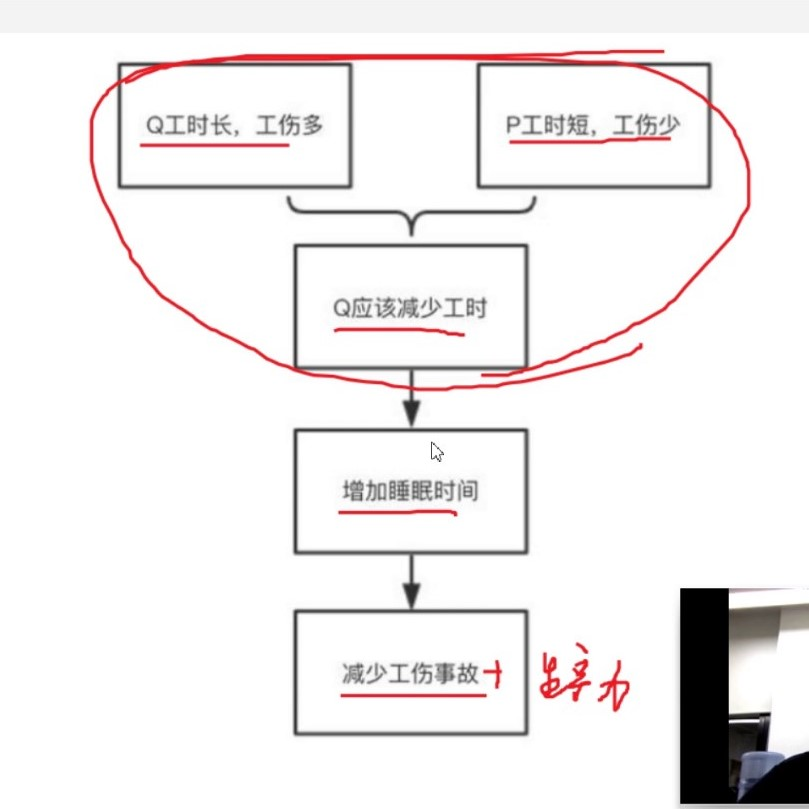
\includegraphics[width=2.925in,height=3.28443in]{illus1.jpg}
\end{center}

\begin{enumerate}
    \item 工伤标准一样吗?如果P很严格,B宽松,那么只是看起来更少。即使一样,上
    报情况一样吗?可能P瞒报了
    \item 工伤和工时一定有关吗?有可能是安全设施不一样,工种不一样。
    \item 即使减少了工时,睡眠时间也不一定增加。比如打游戏。
    \item 即使睡眠时间增加了,事故也不一定会减少。工作内容在将来可能会发生变化。
\end{enumerate}

\subsection{进阶}
首先看argument刷题营,总结所有的简洁提纲。如果时间不太够了或者不想研究黑皮书了。那么自己整理一张表,根据题目重复的次数来排序。先从重复最多的开始(60.用油传统,Consolidated
Company那篇)。根据上述练习方式进行练习。依次往下写。AEQ三种direction几乎是相通的,但explanation不一样,有些问题是不能放到explanation里写的。如果重复题目中有explanation,一定要额外想一想简洁提纲,有精力可以写一写,但考虑到explanation本来数量就不多,所以可以不用写英文全文。

\subsection{上考场}
\begin{enumerate}
    \item 大部分题目简洁提纲比较熟悉,可以不用把所有题目都看完,因为上考场之后,
    就算见过题目,也很难记得清清楚楚自己的简洁提纲具体内容是啥,但是留个印象是十
    分重要的!!!知道大概有哪些问题可以写,所以只要锻炼出3 分钟之内列出一个
    argument简洁提纲的能力就可以了。
    \item 25分钟内能翻译完一篇中文范文(黑皮书上的)。允许对照着中文直接翻译,25
    分钟内至少敲500字。考场上一紧张就是30分钟敲500字了。
\end{enumerate}

\textbf{考场答题步骤:}
\begin{enumerate}
    \item 看题目,必须全看一遍。同时必须看direction,千万别忘了。
    \item 根据印象或者现场画逻辑图。
    \item 找问题,列出简洁提纲。
    \item 疯狂敲字直到时间结束。
\end{enumerate}

\subsection{注记}
\begin{enumerate}
    \item 写英文全文的时候,如果遇到自己想不出来怎么写的英文,一定要标记,同时必须找一个虽然很蠢但能表达意思的表达写上去,不允许查字典。写完了之后再回头去找这个地方,用百度翻译查应该怎么写。
    \item 用百度翻译的时候,直接去找例句,看看例句里面怎么表达的。然而,我必须要提出警告,很多例句来源于中国人写的英文论文(比如你可以从来源中发现wanfang等字眼),可能是错的。所以最稳妥的还是黑皮书和讲义范文,其次是那些来源于字典的例句。网络例句尽量少看。
\end{enumerate}

没有反馈的写作练习,意义不大。写完一定要自己(对照着范文)批改,或者找比你厉害的人批改。

\section{Issue}
如果对写作分数要求不高,就直接放弃吧。只要不跑题,苟个3分就行了。

\begin{quote}
连琦叔都喊太难了的东西,佛一佛算了。
\end{quote}

微臣给的Issue范文并不多,黑皮书上有20篇,但其中的大多数都完全没有参考价值,比如讨论as
we acquire more knowledge, comprehensible, complex,
mystery那一篇,根本不可能在考场上30分钟写这么一篇好文章的(事实上我根本没看懂这篇范文)。实际上比较有参考意义的及篇范文,是在onepass讲义上的最后,有几篇onepass课程上现场写作的issue范文,那几篇是很有参考价值的,不但思路完全贴合课上教的写作方法,同时语言没有很太花里胡哨,是有模仿可行性和意义的。

如果要准备issue的话,首先一定要听onepass课,琦叔会告诉你怎么写issue,扣题+扣direction。之后是onepass讲义上的那几篇issue范文,同argument一样,先自己写简洁提纲,再对照范文,最后修改自己的简洁提纲,写出一篇完整的英文作文(掐表30分钟),最后再对照范文进行修改。这个过程中一定要学会找同义重复,把它们都积累下来。

如果还有余力,就研读一下黑皮书上的范文。优先准备那些重复次数多的题目(在onepass讲义最后一页有issue题目3s版本和分类),优先写好简洁提纲,其次是写英文全文并对照黑皮书范文。

\textbf{考场答题步骤:}
\begin{enumerate}
\item 看题目,必须全看一遍。同时必须看direction,千万别忘了。
\item 2分钟内想出论点。
\item 迅速想出例子,想不出来就胡编,用琦叔告诉你的虚拟例子,另外一定要贴合你
的论证逻辑!千万不要一慌就忘了。
\item 疯狂敲字直到时间结束。
\end{enumerate}

\chapter{经历分享}
最后说说我自己的经历。

\section{考试概况}
成绩162+170+4.5,Q加试。

Issue是beginner和expert那篇,Argument是BF两家公司防腐能力的那篇。Verbal碰到了2-3道填空原题,阅读文章碰到2篇几乎一样的文章,但题目和做过的不一样。成绩诊断V部分medium阅读错4个,长文章错了两个,填空错了3个。Hard部分阅读没错,填空错了4个。总共错了11个,162分。Q全对。

\section{备考经历}
我前期背单词用的是anki,后来背书,再到后来用excel词表,发现词表最适合我。我背单词其实很不扎实,就背了15遍左右吧,而且只记住了中文意思,英文意思基本没记。但我对高频单词的考法非常熟练,这主要归功于认真研读填空题目的解析和做24套。

3000里面还有六七百个词我不认识,中文都想不出来意思,但这并不影响考162,那些单词,我做的题目中只见过1次甚至一次都没见过。

长难句使用大黄的方法才读通的,看完大黄再做阅读确实会轻松很多,但初期中期和后期都仍然不轻松。

填空方面,我24套做了3遍,36套只做了前18个exercise。金皮书做了1遍,1200题里面只做了41-53,64-83,111-120。相比较于很多考生,我做的题真的很少。一般的考生都是1200题刷了至少1遍的。然而考162的人比例并不大。所以我一再强调,先做有解析的题目,弄懂比做要重要的多。填空我的正确率一般在80\%左右,111-120这部分只有65\%。

阅读方面,白皮书只做了7篇,50篇讲义做完了,200篇做了前60。我做的阅读题更少,但从一开始我做阅读正确率就能达到80\%左右。因此我强调大黄一定要看。

Verbal方面总结,我属于阅读比填空强的类型。单词背的很不熟练,填空完全是靠阅读的方法苟出来的。

数学我只看了onepass里面刘新言老师的知识点回顾。之后做了500题讲义中的精选200题和真170中的前50,剩下的题目懒得做了。反正就随随便便170。关键就是要读懂题目+细心!细心!细心!

AW部分我花了很大功夫。Argument刷完了90\%的题目,简洁提纲也全都写完了,英文全篇大约写了20篇。Issue刷了10几道黑皮书和微臣讲过的题目,英文全篇写了不到10篇。我主要优势是打字快,所以考场上碰到那篇比较好写的,issue敲了500多。

\section{建议}
另外,在备考过程中,大家要牢记``常听常熟,常记常新''的道理。这一点体现在做题上就是经典的题目要多做,不厌其烦地做烂,比如24套。体现在听课上就是,那些简单的课,如长难句/阅读/填空方法论视频,不要嫌简单就不看。此外如果你经济条件允许,微臣的课你都听听,即使是上过一遍onepass,再上一遍也没有什么不好的。

我也要额外强调一下安神班,尽管你可能会觉得安神班就是打广告用的,讲的东西肯定都会,但我仍然建议每期都听,反正9.9也不贵,而且还讲本月高频题目,作文那部分就是疯狂给你灌输必须要牢记的点。那些爆品福利课更要好好听。直播听课不仅仅是互动方便,有不会的可以马上问老师,更重要的是老师重复的给你讲一些关键点,你会记得很牢固。此外,直播听课也能提高学习效率,毕竟如果看录屏可能就快放甚至随便跳了,你可能会错失一些穿插讲解的小技巧。当然,如果你没有那么多时间,就算了。

我认为GRE里最有价值的东西是微臣的阅读方法和英文写作技巧,这是不止能提高GRE成绩的东西,更是能帮助我们克服学术障碍中的英文部分的利器。

最后再说一句,微臣家方法是互通的,学了GRE可以吊打托福,除了听力全都免考,考试如同van优戏。因此也强烈建议你们托福也用微臣的方法,不但简单,而且快速有效。

简单说三点:听力千万\textbf{别记笔记};口语在准备的时候就\textbf{直接说},不要补笔记;综合写作直接抄听力和阅读原文,不用瞎拽自己的语言。

了解更多详情可以听听托福的各个onepass课。

\begin{center}\Huge\heiti
\fbox{祝大家早日考出GRE!}
\end{center}

\end{document}
